\documentclass[10pt, handout, envcountsect]{beamer} % text size parameter 10, ratio parameter, handout (in case of need to share)

\usetheme{Madrid} % view themes and colors at https://www.overleaf.com/learn/latex/Beamer#Reference_guide
% \usecolortheme{seahorse}

% \usepackage{pgfpages} % handouts (in case of need to share)
% \pgfpagesuselayout{4 on 1}[a4paper, border shrink=5mm]

\setbeamertemplate{navigation symbols}{} % hides navigation buttons at buttom 
%\setbeamertemplate{footline}[frame number]{} % gets rid of bottom navigation bars
\setbeamercovered{transparent} % makes transparent paramters

\setbeamertemplate{headline}{} % hides navigation bar on top

\usepackage{graphicx} % Required for inserting images
\title[Paper Review]{Paper Review}
\subtitle{
\large{The Description Length of Deep Learning Models}
\\
\vspace{3pt}
\normalsize{Léonard Blier, Yann Ollivier}
}
\author{Gavrilyuk Alexander}
\date{October 2023}

\begin{document}

\maketitle

% ------------------------------

\begin{frame}{Outline}

\tableofcontents

\end{frame}

\section{Motivation $\&$ Problem statement}
% ------------------------------

\begin{frame}{Motivation $\&$ Problem statement}
\begin{itemize}
    \item How much do current deep models actually compress data? (Explicit measurement)
\end{itemize}

% $$
% \boldsymbol{g}^{(\ell)}(\boldsymbol{x})=\boldsymbol{W}^{(\ell)} \boldsymbol{h}^{(\ell-1)}(\boldsymbol{x}), \quad \boldsymbol{h}^{(\ell)}(\boldsymbol{x})=\phi\left(\boldsymbol{g}^{(\ell)}(\boldsymbol{x})\right).
% $$

\begin{figure}[h]
    \centering
    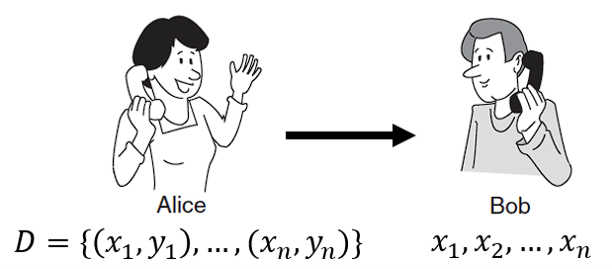
\includegraphics[width=7.5cm,]{fig1.png}
    \caption{Supervised learning illustration when the input data $x$ is public but predictions $y$ are needed.}
    % \label{}
\end{figure} 
    
\end{frame}


\section{Theory}
% ------------------------------
\begin{frame}{Definitions $\&$ Assumption on neural network}

\begin{definition}[Notation]
Let $X$ be the input space and $Y = \{1,...,K\}$ the output space. The dataset is 
$D := \{(x_1, y_1), (x_2, y_2)\}$
A model for supervised learning is defined as a conditional probability distribution
$p(y|x)$, such as for each $x \in X, \sum_{y \in Y}{p(y|x) = 1}$

A model class is a set of models depending one some parameter $\theta$:
$
M = \{p_\theta , \theta \in \Theta\}
$

The Kullback–Leibler divergence between two distributions is 
$$
KL(\mu||\nu) = E_{X \sim \mu}[\log_{2} \frac{\mu(x)}{\nu(x)}]
$$

\end{definition}

\begin{definition}[Shannon–Huffman code]
Suppose that Alice and Bob have agreed in advance on a
model $p$, and both know the inputs $x_{1:n}$. Then there exists a code to transmit the labels $y_{1:n}$ losslessly with codelength
$$
L_p(y_{1:n}|x_{1:n}) = - \sum_{i=1}^{n}\log_{2}p(y_i|x_i)
$$

\end{definition}
    
\end{frame}

% ------------------------------

\begin{frame}{Studied encodings}

\begin{definition}[Uniform encoding]
The uniform distribution $p_{unif}(y|x) = \frac{1}{K}$ over K classes does not require any learning from the data, thus no additional information has to be transmitted. Using $p_{unif}(y|x)$ yields a codelength

$$
L^{unif}(y_{1:n}|x_{1:n}) = n\log_{2}K
$$
    
\end{definition}

\begin{definition}[Two-Part Encodings]
Assume that Alice and Bob have first agreed on a model class
$(p_{\theta})_{\theta \in \Theta}$. Let $L_{param}(\theta)$ be any encoding scheme for parameters $\theta \in \Theta$. Let $\theta^{*}$ be any parameter. The corresponding \emph{two-part codelength} is

$$
L_{\theta^{*}}^{2-part}(y_{1:n}|x_{1:n}) := L_{param}(\theta^{*}) + L_{p_{\theta^{*}}}(y_{1:n}|x_{1:n}) = L_{param}(\theta^{*}) - \sum_{i=0}^{n}\log_{2}p_{\theta^{*}}(y_{i}|x_{i})
$$

    
\end{definition}
    
\end{frame}

% ------------------------------

\begin{frame}{Studied encodings}

\begin{definition}[Variational and Bayesian Codes]
Assume that Alice and Bob have agreed on a model class $(p_{\theta})_{\theta \in \Theta}$ and a prior $\alpha$ over $\Theta$. Then for any distribution $\beta$ over $\Theta$, there exists an encoding with codelength

$$
L^{var}_{\beta}(y|x) = KL(\beta||\alpha) + E_{\theta\sim\beta}[L_{p_{\theta}}(y_{1:n}|x_{1:n})] = KL(\beta||\alpha) - E_{\theta\sim\beta}[\sum_{i=0}^{n}\log_{2}p_{\theta}(y_{i}|x_{i})]
$$

The variational bound $L^{var}_{\beta}$ is an upper bound for the Bayesian description length bound of the Bayesian model $p_{\theta}$ with parameter $\theta$ and a prior $\alpha$. Considering the Basyesian distribution of y, an associated code with model $p_{\theta}: L^{Bayes}(y_{1:n}|x_{1:n}) = -\log_{2}p_{Bayes}(y_{1:n}|x_{1:n})$ is provided:

$$
L_{\beta}^{var}(y_{1:n}|x_{1:n}) \ge L^{Bayes}(y_{1:n}|x_{1:n})
$$
    
\end{definition}
    
\end{frame}

% ------------------------------

\begin{frame}{Studied encodings}

\begin{definition}[Prequential or Online Code]
Lets call $p$ a \emph{prediction strategy} for predicting the labels in $Y$ knowing the inputs in $X$ if for all $k$, $p(y_{k+1}|x_{1:k+1}, y_{1:k})$ is a conditional model. Any prediction strategy p defines a model on the whole dataset:

$$
p^{preq}(y_{1:n}|x_{1:n}) = p(y_1|x_1) * p(y_2|x_{1:2}, y_1) * ... * p(y_n|x_{1:n}, y_{1:n-1})
$$

Let $(p_{\theta})_{\theta \in \Theta}$ be a DL model. We assume that we have a learning algorithm which computes, from any number of data samples $(y_{1:k}|x_{1:k})$, a trained parameter vector $\hat{\theta}(x_{1:k}, y_{1:k})$. This yields the following description length:

$$
L^{preq}(y_{1:n}|x_{1:n}) = t_1\log_{2}K + \sum_{s=0}^{S-1} - \log_{2}p_{\hat{\theta}_{t_s}}(y_{t_s+1:t_{s+1}}|x_{t_s+1:t_{s+1}})
$$
where for each $s, \hat{\theta}_{t_s} = \hat{\theta}(x_{1:t_s}, y_{1:t_s})$ is the parameter learned on data samples 1 to $t_s$.
    
\end{definition}
    
\end{frame}
% ------------------------------
\section{Experiment}
% ------------------------------
\begin{frame}{Experiment}


\begin{figure}[h]
    \centering
    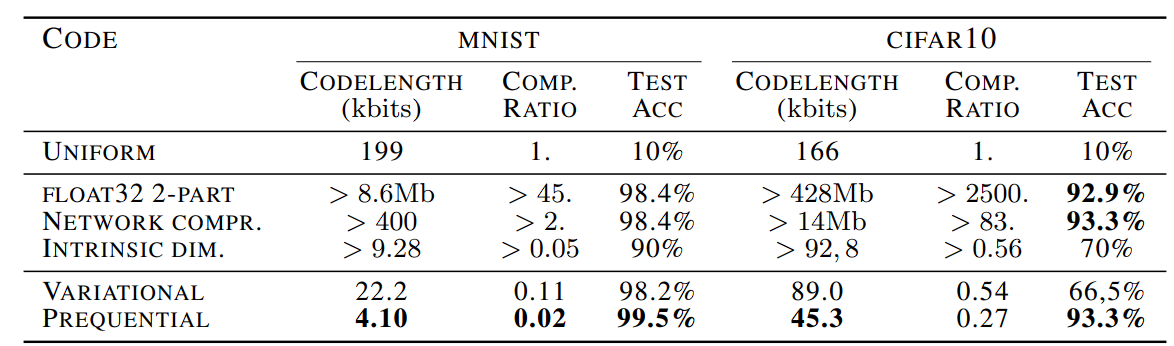
\includegraphics[width=12cm,]{fig2.png}
    \caption{Compression bounds via Deep Learning. The \emph{codelength} is the number of bits necessary to send the labels to someone who already has the inputs. This codelength includes the description length of the model. The \emph{compression ratio} for a given code is the ratio between its codelength and the codelength of the uniform code. The \emph{test accuracy} of a model is the accuracy of its predictions on the test set.}
    % \label{}
\end{figure} 
    
\end{frame}

% ------------------------------

\begin{frame}{Experiment}


\begin{figure}[h]
    \centering
    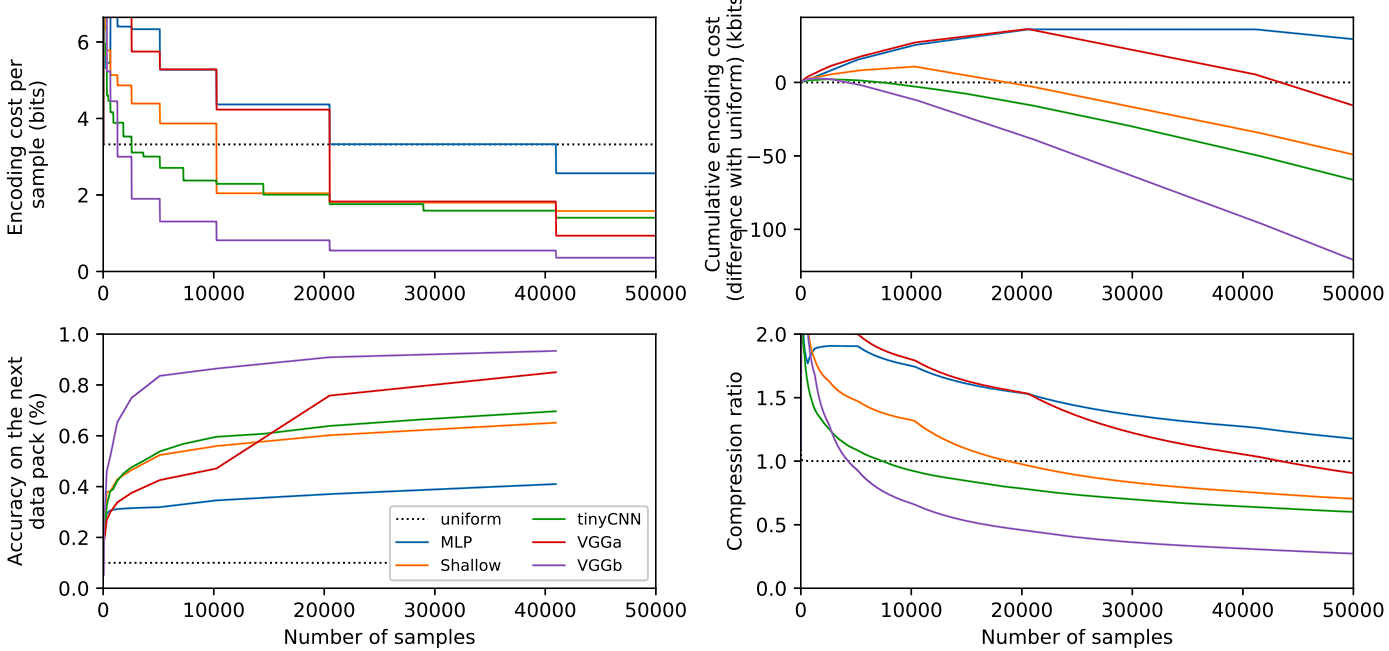
\includegraphics[width=12cm,]{fig3.png}
    \caption{Prequential code results on CIFAR. Results of prequential encoding on CIFAR with 5 different models: a small Multilayer Perceptron (MLP), a shallow network, a small convolutional layer (tinyCNN), a VGG-like network without data augmentation and batch normalization (VGGa) and the same VGG-like architecture with data augmentation and batch normalization (VGGb).}
    % \label{}
\end{figure} 
    
\end{frame}

% ------------------------------


\end{document}
